\documentclass{standalone}
% tkz-fct: parabola sampled through the fp fixed-point evaluator.
% \tkzFct itself draws via gnuplot (runsystem), which the worker cannot
% run; the fp family (fp.sty + its fp-*.sty modules, required at load) is
% the in-engine evaluator, exercised here through \FPeval + \tkzFctPt.
% Two fp/tkz quirks the sampling has to respect: fp cannot take a negative
% macro as a bare operand (hence (\x)*(\x) and (-2)+...), and \tkzFctPt
% restores \tkz@init@xstep from \tkz@tmp@xstep, which only \tkzFct ever
% sets — pre-establish that invariant once after \tkzInit.
\usepackage{tkz-fct}
\begin{document}
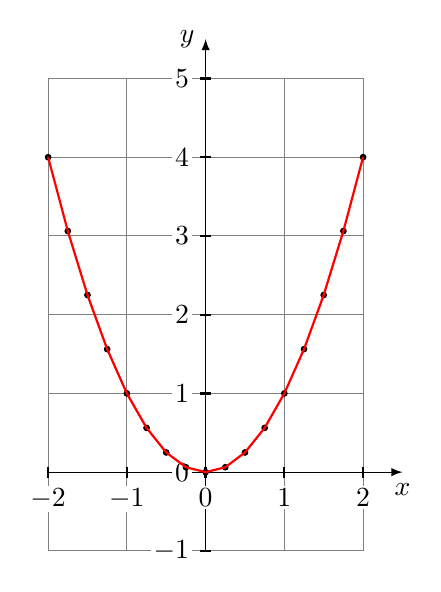
\begin{tikzpicture}
\tkzInit[xmin=-2,xmax=2,ymin=-1,ymax=5]
\tkzGrid
\tkzAxeXY
\makeatletter\let\tkz@tmp@xstep\tkz@init@xstep\makeatother
\foreach \i in {0,...,16}{%
  \FPeval\xv{(-2)+\i*0.25}%
  \tkzFctPt{(\x)*(\x)}(\xv){P\i}%
}
\draw[red,thick] (P0) \foreach \i in {1,...,16}{ -- (P\i) };
\end{tikzpicture}
\end{document}
